% Preamble ==================================================================
\documentclass[11pt]{article}
\usepackage{geometry}
\geometry{verbose,tmargin=2.5cm,bottom= 1.5cm,lmargin=2.5cm,rmargin=2.5cm}
\usepackage{float}
\usepackage{graphicx}
\usepackage{amsmath}
\usepackage{amssymb}
\usepackage{enumitem}
\usepackage{mathtools}


\numberwithin{equation}{section}

\usepackage{titlesec,dsfont}

%Format section heading style
\usepackage{sectsty}
\sectionfont{\sffamily\bfseries\small}
\subsectionfont{\sffamily\small\slshape}
\subsubsectionfont{\sffamily\small\itshape}
\paragraphfont{\sffamily\small\textbf}


%Put period after section number
\makeatletter
\def\@seccntformat#1{\csname the#1\endcsname.\quad}
\makeatother


%Format captions
\usepackage[ labelsep=period, justification=raggedright, margin=10pt,font={small},labelfont={small,normal,bf,sf}]{caption}

\setlength{\parskip}{0ex} %No space between paragraphs.

\renewcommand{\familydefault}{\sfdefault}

\newcommand\indep{\protect\mathpalette{\protect\independenT}{\perp}}
\def\independenT#1#2{\mathrel{\rlap{$#1#2$}\mkern2mu{#1#2}}}

%PUT ME LAST--------------------------------------------------
\usepackage[colorlinks=true
,urlcolor=black
,anchorcolor=blue
,citecolor=blue
,filecolor=blue
,linkcolor=black
,menucolor=blue
,linktocpage=true
,pdfproducer=medialab
,pdfa=true
]{hyperref}

\makeatother %Put this last of all


\newcommand{\defeq}{\coloneqq}
\newcommand{\overbar}[1]{\mkern 1.5mu\overline{\mkern-1.5mu#1\mkern-1.5mu}\mkern 1.5mu}

%Preamble end--------------------------------------------------


\begin{document}



\begin{flushleft}
\textbf{\Large Causal inference cheat sheet}
\end{flushleft}

\begin{flushleft}
Author: Juvid Aryaman

Last compiled: \today
\end{flushleft}


\section{Basic probability}

\begin{itemize}[noitemsep]
\item Law of total probability: $P(A) = \sum_i P(A, B_i)$ (a.k.a. marginalizing over $B$)
\item Chain rule of probability: $P(A,B) = P(A|B) P(B)$
\item Thus, $P(A) = \sum_i P(A|B_i) P(B_i)$
\item Expectation: $E(g(X)) = \sum_x g(x) P(x)$
\item Conditional mean: $E(X|Y) = \sum_x x P(x|y)$
\item Variance: $\sigma_X^2 = E[(X - E(x))^2]$
\item Covariance: $\sigma_{XY} = E[(X-E(X))(Y-E(Y))]$
\item Correlation coefficient: $\rho_{XY}=\sigma_{XY}/(\sigma_X \sigma_Y)$
\item Regression coefficient of $X$ on $Y$: $r_{XY} = \rho_{XY} \sigma_X/\sigma_Y = \sigma_{XY}/(\sigma_Y^2)$ (for the equation $X = r_{XY} Y + c + \mathcal{N}(0, \sigma^2)$)
\item Conditional independence: $(X \indep Y | Z) \iff P(x|y,z) = P(x|z) $
\end{itemize}

The recursive decomposition of the joint distribution into parents which characterises Bayesian networks is
\begin{equation}
P(x_1, ..., x_n) = \prod_i P(x_i|pa_i) \label{eq:bayes-net-char}
\end{equation}

\subsection{$d$-separation (blocking) in Bayesian networks} \label{sec:blocking}
A path $p$ is $d$-separated (or blocked) by a set of notes $Z$ if and only if
\begin{enumerate}[noitemsep]
\item $p$ contains a chain $i \rightarrow m \rightarrow j$ or a fork $i \leftarrow m \rightarrow j$ such that the middle node $m$ is in $Z$, or
\item $p$ contains a collider $i \rightarrow m \leftarrow j$ such that the middle node $m$ is not in $Z$ and such that no descendant of $m$ is in $Z$
\end{enumerate}
where an arrow $pa_j \rightarrow x_j$ denotes part of a directed acyclic graph (DAG) in which variables are represented by nodes and arrows are drawn from each node of the parent set $PA_j$ towards the child node $X_j$.

\paragraph{Probabilistic implications of $d$-separation} 
Consequently, if $X$ and $Y$ are $d$-separated by $Z$ in a DAG $G$, then $(X \indep Y | Z)$ in every distribution compatible with $G$. Conversely, if $X$, $Y$, and $Z$ are \textit{not} $d$-separated by $Z$ in a DAG $G$ then $X$ and $Y$ are dependent conditional on $Z$ in almost all distributions compatible with $G$ (assuming no parameter fine-tuning).

\section{Functional causal models}
A functional causal model consists of a set of equations of the form
\begin{equation}
x_i = f_i(pa_i, u_i), \quad i=1,...,n \label{eq:func-caus-mod}
\end{equation}
where $pa_i$ are the set of variables (parents) that directly determine the value of $X_i$ and $U_i$ represents errors (or ``disturbances'') due to omitted factors. When some disturbances $U_i$ are judged to be dependent, it is customary to denote such dependencies in a causal graph with double-headed arrows. If the causal diagram is acyclic, then the corresponding model is called \textit{semi-Markovian} and the values of the variables $X$ are uniquely determined by those of the variables $U$. If the error terms $U$ are jointly independent, the model is called \textit{Markovian}.

Linear structural equation models obey
\begin{equation}
x_i = \sum_{k \neq i} \alpha_{ik} x_k + u_i, \quad i=1,...,n 
\end{equation}
In linear models, $pa_i$ corresponds to variables on the r.h.s.\ of the above equation where $\alpha_{ik} \neq 0$.

\subsection{Counterfactuals in functional causal models: An example}
Consider a randomized clinical trial, where patients are/are not treated $X \in \{0,1\}$. We also observe whether the patients die after treatment $Y\{0,1\}$. We wish to ask the question: did the patient die \textit{because of} the treatment, \textit{despite} the treatment, or \textit{regardless} of the treatment.

Assume $P(y|x) = 0.5$, and therefore $P(y,x)=0.25$ for all $x$ and $y$. We can write two models with the same joint distribution

\textit{Model 1 (treatment no effect):}
\begin{align}
&x=u_1\\
&y=u_2\\
&P(u_1=1) = P(u_2=1)= \frac{1}{2}
\end{align}


\textit{Model 2 (treatment has an effect):}
\begin{align}
&x=u_1\\
&y=xu_2 + (1-x)(1-u_2)\\
&P(u_1=1) = P(u_2=1)= \frac{1}{2}
\end{align}

Let $Q$=fraction of deceased subjects from the treatment group who would not have died had they not taken the treatment. In model 1, $Q=0$ since $X$ has no effect on $Y$. In model 2, subjects who died ($y=1$) and were treated ($x=1$) must correspond to $u_2=1$. If $u_2=1$ then the only way for $y=0$ is for $x=0$. I.e. if you are a patient for whom $u_2=1$ then the only way not to die is to not take the treatment, so the treatment caused your death. So $Q=1$.

Consequence 0: joint probability distributions are insufficient for counterfactual computation

Consequence 1: stochastic causal models are insufficient for counterfactual computation

Consequence 2: functional causal models are sufficient to define and compute counterfactual statements.

\subsection{General method to compute counterfactuals}
Given evidence $e=\{X_{obs}, Y_{obs}\}$, to compute probability of $Y=y$ under hypothetical condition $X=x$ apply the following steps:
\begin{enumerate}[noitemsep]
\item Abduction: Update the probability of disturbances $P(u)$ to obtain $P(u|e)$
\item Action: Replace the equations corresponding to variables in the set $X$ by the equations $X=x$
\item Prediction: Use the modified model to compute the probability $Y=y$.
\end{enumerate}

\section{Causal Bayesian networks}
Given two disjoint sets of variables $X$ and $Y$, the \textbf{causal effect} of $X$ on $Y$, denoted as $P(y|\hat{x})$ or $P(y|do(x))$, is the probability of $Y=y$ by deleting all equations from Eq.\eqref{eq:func-caus-mod} where variables $X$ are on the l.h.s., and substituting $X=x$ in the remaining equations.

This corresponds to mutilating the DAG such that all arrows pointing directly to $X_i$ are removed. \textbf{Amputation is the difference between seeing and doing}.

For an atomic intervention, we get the \textit{truncated factorization} formula
\begin{equation}
P(x_1,...,x_n|\hat{x}'_i)=\begin{dcases}
\prod_{j\neq i} P(x_j|pa_j) \quad &\text{if}\ x_i = x_i'\\
0 &\text{if}\ x_i \neq x_i'
\end{dcases}
\end{equation}
The $j\neq i$ denotes the removal of the term $P(x_i|pa_i)$ from Eq.\eqref{eq:bayes-net-char} (i.e. amputation). A $do(x_i)$ is a severely limited sub-space of the full joint distribution, since the distribution only has support where the intervention variable $x_i$ is equal to its particular intervention value $x_i'$, rather than a continuum of values in Eq.\eqref{eq:bayes-net-char}.

Multiplying and dividing by $P(x'_i|pa_i)$ yields
\begin{equation}
P(x_1,...,x_n|\hat{x}'_i)=\begin{dcases}
P(x_1,...,x_n|x_i',pa_i)P(pa_i) \quad &\text{if}\ x_i = x_i'\\
0 &\text{if}\ x_i \neq x_i'
\end{dcases}
\end{equation}
Marginalization of the above leads to the following theorem.

\paragraph{Adjustment for direct causes} 
Let $PA_i$ denote the set of direct causes of variable $X_i$, and let $Y$ be any set of variables disjoint of $\{X_i \cup PA_i \}$. The causal effect of $do(X_i=x_i')$ on $Y$ is
\begin{equation}
P(y|\hat{x}_i') = \sum_{pa_i} P(y | x'_i, pa_i) P(pa_i)
\end{equation}
where $P(y|x_i', pa_i)$ and $P(pa_i)$ are preintervention probabilities. This is called ``adjusting for $PA_i$''.


\paragraph{Identifiability}
Causal quantities are defined relative to a causal model $M$, not the joint distribution $P_M(v)$ over the set of observed variables $V$. Non-experimental data provides information about $P_M(v)$ alone, and several graphs can give rise to the same $P_M(v)$. Thus, not all quantities are unambiguously \textbf{identifiable} from observational data, \textbf{even with infinite samples}. Added assumptions by specifying a particular $M$ can provide enough details to compute quantities of interest without explicating $M$ in full.

Theorem 3.2.5: Given a causal diagram $G$ of any Markovian model in which a subset of variables $V$ are measured, the causal effect $P(y|\hat{x})$ is identifiable whenever $\{X \cup Y \cup PA_X\} \subseteq V$. I.e. \textit{all parents of the cause are necessary to estimate the causal effect}.

\section{Inferring causal structure}
\begin{itemize}
\item IC algorithm is for inferring causal structure given observational data when there are no latent variables
\item IC* algorithm is for inferring causal structure given observational data when there are latent variables. The PC algorithm is apparently more contemporary (see Spirtes et al 2010)
\item There are local criteria for potential cause and genuine cause
\item Spurious association: $X$ and $Y$ are spuriously associated if they are dependent in some context and there exists a latent common cause, as exemplified in the structure $Z_1 \rightarrow X \rightarrow Y \leftarrow Z_2$
\item NOTEARS (Zheng et al.\ 2018) casts the structure learning problem as a continuous optimization problem over real matrices to avoid the superexponential combinatorial explosion with number of variables.
\end{itemize}

\section{Adjusting for confounding bias}

When seeking to evaluate the effect of one factor ($X$) on another ($Y$), we should ask \textbf{whether} we should \textit{adjust} for possible variations in other factors ($Z$, known as ``covariates'', ``concomitants'' or ``confounders''). This becomes apparent in \textbf{Simpson's paradox}: any statistical relationship between two variables may be reversed by including additional factors in the analysis.

\subsection{The back-door criterion}
This criterion demonstrates how confounders that \textit{affect} the treatment variable can be used to facilitate causal inference.

\begin{figure}
\begin{center}
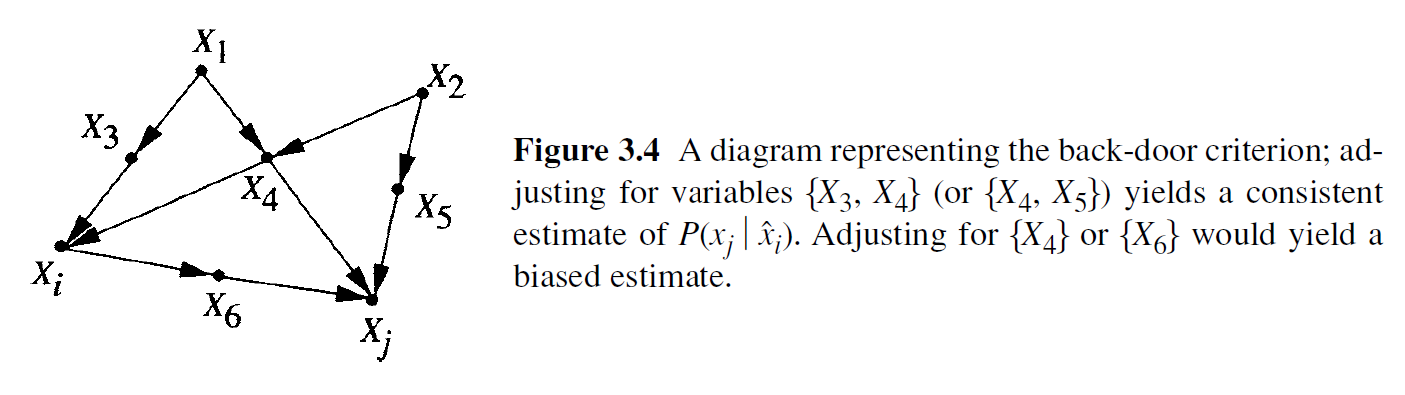
\includegraphics[width=0.8\columnwidth]{figures/back-door.png}  
\end{center}
\caption{Example of the back-door criterion
}
\label{Fig:front_door}
\end{figure}

\paragraph{Back-door} 
A set of variables $Z$ satisfy the back-door criterion relative to an ordered pair of variables ($X_i$,$X_j$) in a DAG $G$ if:
\begin{enumerate}[noitemsep]
\item no node in $Z$ is a descendant of $X_i$; and
\item $Z$ blocks every path between $X_i$ and $X_j$ that contains an arrow into $X_i$
\end{enumerate}
Similarly, if $X$ and $Y$ are two disjoint subsets of nodes in $G$, then $Z$ satisfies the back-door criterion relative to $(X,Y)$ if it satisfies the criterion relative to any pair $(X_i, X_j)$ such that $X_i \in X$ and $X_j \in Y$.

\paragraph{Back-door adjustment}
If a set of variables $Z$ satisfies the back-door criterion relative to $(X,Y)$, then the causal effect of $X$ on $Y$ is identifiable and is given by
\begin{equation}
P(y|\hat{x}) = \sum_z P(y|x,z)P(z).
\end{equation}
This corresponds to partitioning the population into groups that are homogeneous relative to Z, assessing the effect of X on Y in each homogeneous group, and then averaging the results. Conditioning in this way means that the observation $X=x$ cannot be distinguished from an intervention $do(x)$.

\subsection{The front-door criterion}
This criterion demonstrates how confounders that are \textit{affected by} the treatment variable can be used to facilitate causal inference.

\begin{figure}
\begin{center}
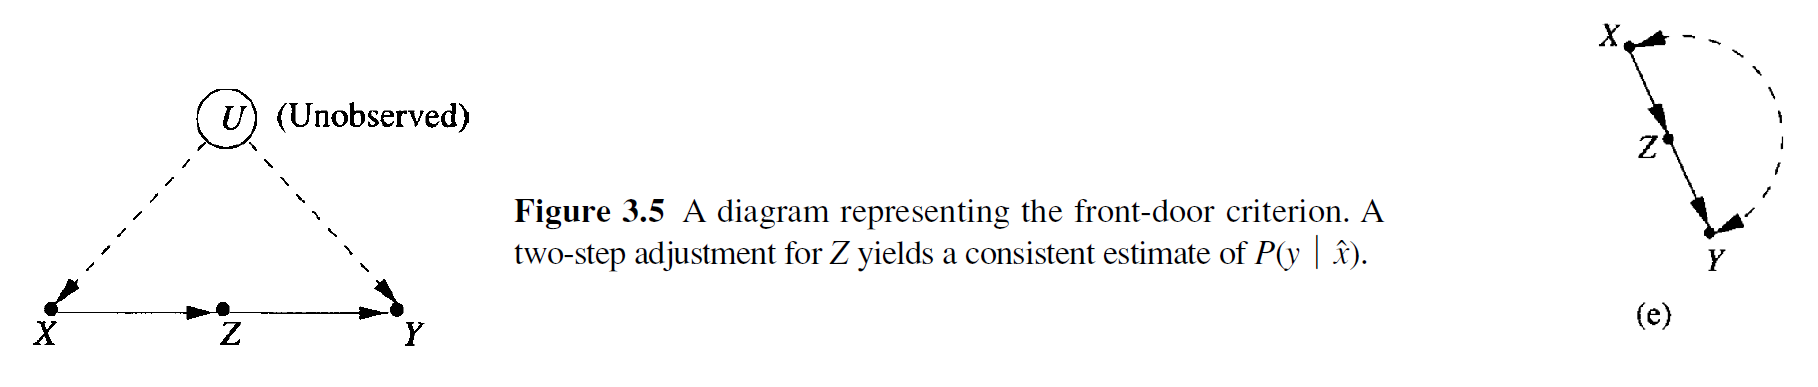
\includegraphics[width=0.8\columnwidth]{figures/front-door.png}  
\end{center}
\caption{(Left) Example of the front-door criterion. The path $X \leftarrow U \rightarrow Y$ denotes an unobserved (latent) unobserved common cause. (Right) This is often represented as a \textbf{bi-directed path}. 
}
\label{Fig:front_door}
\end{figure}

\paragraph{Front-door} 
A set of variables $Z$ satisfy the front-door criterion relative to an ordered pair of variables $(X, Y)$ if:
\begin{enumerate}[noitemsep]
\item $Z$ intercepts all directed paths from $X$ to $Y$; 
\item there is no unblocked back-door path from $X$ to $Z$; and
\item all back-door paths from $Z$ to $Y$ are blocked by $X$.
\end{enumerate}

\paragraph{Front-door adjustment}
If $Z$ satisfies the front-door criterion relative to $(X, Y)$ and if $P(x, z) > 0$, then the causal effect of $X$ on $Y$ is identifiable and is given by
\begin{equation}
P(y|\hat{x}) = \sum_z P(z|x) \sum_{x'} P(y|x',z)P(x')
\end{equation}

Conditions (2) and (3) of the front-door definition are overly restrictive: e.g. nested combinations of back-door and front-door conditions are permissible (see Section~\ref{sec:do-calc} for a more general set of conditions).

\section{Do-calculus} \label{sec:do-calc}

The back-door and front-door criteria do not provide a complete set of rules for when/how causal effects can be computed. Do-calculus sidesteps the need for algebraic manipulation and provides a complete set of inference rules by which probabilistic sentences involving interventions and observations can be transformed into other such sentences, allowing a method of deriving/verifying claims about interventions. The aim is to compute causal effect expressions for $P(y|\hat{x})$ where $Y$ and $X$ are subsets of variables. When $P(y|\hat{x})$ can be reduced to an expression involving observable probabilistic quantities, we say that the causal effect of $X$ on $Y$ is \textbf{identifiable}.

\subsection{Notation}
\begin{itemize}[noitemsep]
\item $G_{\overline{X}}$ = graph obtained by deleting from $G$ all arrows pointing into nodes in $X$
\item $G_{\underline{X}}$ = graph obtained by deleting from $G$ all arrows pointing out of nodes in $X$
\item $G_{\overline{X}\underline{Z}}$ = graph obtained by deleting from $G$ all arrows pointing into nodes in $X$ and out of nodes in $Z$
\item $P(y|\hat{x},z) \defeq P(y,z|\hat{x}) / P(z|\hat{x})$, meaning the probability of observing $Y=y$ given an \textit{intervention} $X=x$ and an \textit{observation} $Z=z$
\end{itemize}

\subsection{Rules}

\paragraph{Rule 1} (Insertion/deletion of observations)
\begin{equation}
P(y|\hat{x}, z, w) = P(y| \hat{x}, w) \quad \text{if}\ (Y \indep Z|X,W)_{G_{{\overline{X}}}}.
\end{equation}

This rule is a reaffirmation of $d$-separation (Section~\ref{sec:blocking}) as a valid test for conditional independence in the distribution resulting from $do(X=x)$. The rule follows from the fact that deleting equations from the system ($G_{{\overline{X}}}$) does not introduce any dependencies among the remaining disturbance terms.


\paragraph{Rule 2} (Action/observation exchange)
\begin{equation}
P(y|\hat{x},\hat{z},w) = P(y|\hat{x},z,w) \quad \text{if}\ (Y \indep Z|X,W)_{G_{{\overline{X}\underline{Z}}}}.
\end{equation}

This rule provides a condition for an external intervention $do(Z=z)$ to have the same effect on $Y$ as the passive observation $Z=z$. The condition amounts to $\{X \cup W\}$ blocking all back-door paths from $Z$ to $Y$ (in $G_{\overline{X}}$), since $G_{\overline{X}\underline{Z}}$ retains all (and only) such paths.

\paragraph{Rule 3} (Insertion/deletion of actions)
\begin{equation}
P(y|\hat{x},\hat{z},w) = P(y|\hat{x},w) \quad \text{if}\ (Y \indep Z|X,W)_{G_{{\overline{X},\overline{Z(W)}}}}
\end{equation}
where $Z(W)$ is the set of $Z$-nodes that are not ancestors of any $W$-node in $G_{\overline{X}}$.

This rule provides conditions for introducing (or deleting) an external intervention $do(Z=z)$ without affecting the probability of $Y=y$. The validity of this rule stems from simulating the intervention $do(Z=z)$ by the deletion of all equations corresponding to the variables in $Z$ (hence $G_{\overline{X} \overline{Z}}$).

\paragraph{Completeness} A quantity $Q=P(y|do(x),z)$ is identifiable if and only if it can be reduced to a \textit{do}-free expression using the above 3 rules.

\paragraph{Identifiability}
A causal effect $q = P(y_1, \dots, y_k| \hat{x}_1, \dots, \hat{x}_m)$ is identifiable in a model characterised by a graph $G$ is there exists a finite sequence of transformations conforming to one of the three rules above that reduces $q$ into a standard (i.e.\ ``hat''-free) probability expression involving observed quantities. 

Whilst a causal effect is not identifiable for \textit{every} joint distribution of variables if this condition is broken, it might be for \textit{some} probability densities. For example, an instrumental variable can yield a causal effect identifiable in a linear model in the the presence of a box pattern, but will not be generally identifiable (see Section 3.5 of Causality).

\paragraph{Complete identifiability condition} A sufficient condition for identifying the causal effect $P(y|do(x))$ is that there exists no bi-directed path (i.e.\ a path composed entirely of bi-directed arcs, see Fig.~\ref{Fig:front_door}) between $X$ and any of its children. Prior to applying this criterion, all nodes which are not ancestors of $Y$ are deleted from the graph (i.e.\ only consider nodes which are on pathways from $X$ to $Y$). 

\section{Actions, plans, and direct effects}

Pearl defines two kinds of intervention:

\begin{itemize}[noitemsep]
\item Act: An intervention which results from a reactive policy, deriving from an agent's beliefs, disposition, and environmental inputs (or the ``outside'')
\item Action: An intervention which results from a deliberative policy, deriving from an agent's free will (or the ``inside''; meditative traditions might not draw such a bright line between these two classifications as a  description of physical reality, but it is no doubt a useful distinction for reasoning about the future when conscious agents are involved)
\end{itemize} 

\subsection{Conditional actions and stochastic policies}
In general, interventions may involve complex policies in which $X$ is made to respond according to e.g. a deterministic functional relationship $x=g(z)$, or more generally through a stochastic relationship whereby $X$ is set to $x$ with probability $P^*(x|z)$. 

Let $P(y|do(X=g(z)))$ denote the distribution of $Y$ prevailing under the policy $do(x=g(z))$. Then,
\begin{align}
P(y|do(X=g(z))) &= \sum_z P(y|do(X=g(z)),z) P(z|do(X=g(z))) \\
&= \sum_z P(y|\hat{x}, z)|_{x=g(z)} P(z) \nonumber \\
&= E_z[P(y|\hat{x},z)|_{x=g(z)}]. \nonumber
\end{align}
Hence, the evaluation of the outcome of an intervention under a complicated conditional policy $P^*(x|z)$ amounts to being able to evaluate $P(y|\hat{x},z)$. The equality $P(z|do(X=g(z))) = P(z)$ stems from the fact that $Z$ \textbf{cannot} be a descendant of $X$: in other words, \textbf{one cannot define a coherent policy of action for $X$ based on an (indirect) effect of $X$ because actions change the distributions of their effects!}

(Aside: I suppose one might argue about whether an agent has any choice over the form of $g(z)$)

\end{document}